\chapter{阿代尔群的自守表示I：一般定义}\label{L4}
\lecturedate{2020/02/26}
\sourcepage{27}
Langlands猜想断言，$n$维不可约Galois表示——即数域$F$的群$\Gal(\overline F/F)$的表示——与$\GL_n(\A_F)$的自守表示\znote{「自守」指函数在 $G(\Q)$ 左作用下的不变性（automorphy）。自守表示把这种不变性提升为 $G(\A)$ 的表示：它是带有整体不变性的一类表示，而非 $G(\A)$ 的任意表示。Galois 表示携带算术信息但缺少解析结构，Langlands 猜想断言两者是同一对象的两面。[来源：Bernstein--Gelbart, \textit{An introduction to the Langlands Program}, Birkh\"auser, 2004, 第 7 章（本讲参考文献）。]}之间存在一一对应。当$n=2$、$F=\Q$时，该猜想成立；粗略地说，在这一情形中，对应通过如下方式建立：
% [Tutor Note: 原书此处用语宽泛；就本书语境而言，已知成立的是 $n=1$ 的类域论情形。]
\begin{figure}[H]\centering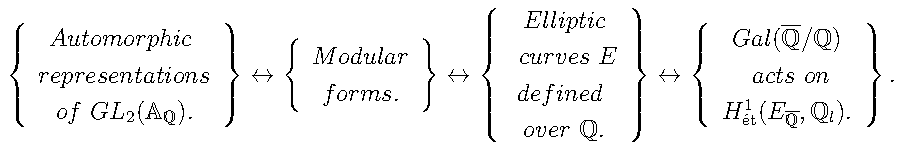
\includegraphics[width=0.7257\paperwidth]{images/L4-p027-correspondence.pdf}\end{figure}
记$\A_F^f$为$\A_F$的有限部分，即$\A_F$投影到$\prod_{\p\text{ 有限}}F_{\p}$所得的像。按照定义，$G(\A_{\Q})$的自守表示是$G(\Q)\backslash G(\A_{\Q})$上某个函数空间$\mathcal A(G)$的子商表示。严格地说，$\mathcal A(G)$并不承载整个$G(\R)$的作用；实际作用于它的是$G(\A_{\Q}^f)\times(K,\g)$，其中$K$为$G(\R)$的极大紧子群，$\g$是$G(\R)$的Lie代数。
% [Tutor Note: 原书 p27 作「$K$ is the maximal compact subgroup of $\A_{\Q}$」；$\A_{\Q}$ 是阿代尔环、没有紧子群这一说法，此处应为 $G(\R)$，译文按 $G(\R)$ 处理。]
\section{阿代尔环作为拓扑环的进一步性质}\label{L4S1}
设$F$为数域，$\p$为$F$的有限素位，$F_{\p}$为$F$在$\p$处完备化得到的局部域，并取规范化离散赋值$v_{\p}$。
\sourcepage{28}
定义绝对值$|x|_{\p}=q^{-v_{\p}(x)}$（$x\ne0$），并令$|0|_{\p}=0$；这里$\OO_{\p}/\p\cong\F_q$，$\OO_{\p}$为$F_{\p}$中的离散赋值环。
% [Tutor Note: 原书 p28 印作 $|x|_{\p}=q^{v_{\p}(x)}$，指数缺负号；乘积公式要求 $|x|_{\p}=q^{-v_{\p}(x)}$，译文按正确写法处理。]
$|\cdot|_{\p}$给出度量，从而在$F_{\p}$及$F_{\p}^\times$上给出拓扑。以下标准事实容易验证。
\begin{property}
\begin{itemize}
\item $F_{\p}$局部紧。
\item $\OO_{\p}$紧。
\item $F_{\p}$和$F_{\p}^\times$都是全不连通的，即非空连通子集只能是单点。
\end{itemize}
\end{property}
若$\p$为无穷素位，它对应于嵌入$\iota_{\p}:F\hookrightarrow\C$。实素位处定义$|x|_{\p}=|\iota_{\p}(x)|$，复素位处定义$|x|_{\p}=|\iota_{\p}(x)|^2$，其中右边为$\C$的通常绝对值。无穷素位处的$\OO_{\p}=F_{\p}$不紧，$F_{\p}$和$F_{\p}^\times$也不全不连通，但$F_{\p}$仍局部紧。

因为$F\subseteq F_{\p}$，所以对$X\in F^\times$，各处的$|X|_{\p}$均有定义。
\originalnumber{1}
\begin{theorem}\label{L4S1O1}\idx{乘积公式}
设$X\in F^\times$，则除至多有限多个$\p$外都有$|X|_{\p}=1$，且$\displaystyle\prod_{\p}|X|_{\p}=1$。
\end{theorem}
\originalnumber{2}
\begin{lemma}\label{L4S1O2}
设$X\in F^\times$，则除至多有限多个$\p$外都有$|X|_{\p}\leq1$。
\end{lemma}
\begin{proof}
$F$的无穷素位只有有限多个，因为$F/\Q$有限，而$\Q$只有一个无穷素位。因此只需考虑有限素位$\p$，此时$|\cdot|_{\p}$是非阿基米德绝对值。设$X\in F$，则$X$在$\Q$上是代数的，故
\[X^m+a_1X^{m-1}+\cdots+a_m=0,\qquad a_1,\ldots,a_m\in\Q.\]
于是
\[|X|_{\p}^m\leq\max\{|a_1|_{\p}|X|_{\p}^{m-1},\ldots,|a_m|_{\p}\}\leq\max\{1,|X|_{\p}^{m-1}\}\max_i|a_i|_{\p}.\]
固定的有理数$a_1,\ldots,a_m$在几乎所有有限素位处都满足$|a_i|_{\p}\leq1$；若此时$|X|_{\p}>1$，上述不等式便给出$|X|_{\p}^m\leq|X|_{\p}^{m-1}$，矛盾。因此$|X|_{\p}\leq1$。
\end{proof}
\sourcepage{29}
\begin{proof}[\eref{定理}{L4S1O1}的证明概要]
由\eref{引理}{L4S1O2}，对几乎所有$\p$，有$|X|_{\p}\leq1$和$|X^{-1}|_{\p}\leq1$，故$|X|_{\p}=1$。再利用规范化赋值在扩张中的性质，将乘积公式归结为$F=\Q$的情形；直接计算即得结论。
\end{proof}
可以定义群同态
\begin{equation}\tag{1.1}\label{L4eq11}
c:\mathbb{I}_F\longrightarrow\R_{>0},\qquad\alpha=(\alpha_{\p})_{\p}\longmapsto\prod_{\p}|\alpha_{\p}|_{\p}.
\end{equation}
\begin{exercise*}\label{L4S1EX1}
证明\eqref{L4eq11}中的$c$良定义，即对所有$\alpha\in\mathbb{I}_F$，右边的乘积都在$\R_{>0}$中有意义。
\end{exercise*}
由\eref{定理}{L4S1O1}，$F^\times\subseteq\ker c=:\mathbb{I}_F^1$。
\originalnumber{3}
\begin{theorem}{弱逼近定理}\label{L4S1O3}\idx{弱逼近定理}
设$|\cdot|_j$（$1\leq j\leq N$）为域$F$上有限个彼此不等价的非平凡绝对值。记$F_j$为集合$F$配上$|\cdot|_j$诱导的拓扑所得的拓扑空间。则$F$经对角嵌入所得的像$\Delta\subseteq\prod_{j=1}^N F_j$在$\prod_{j=1}^N F_j$中稠密。
\end{theorem}
\originalnumber{4}
\begin{note}[L4S1O4]
\eref{定理}{L4S1O3}等价于如下陈述：给定任意$x_j\in F$（$1\leq j\leq N$）和任意实数$\varepsilon>0$，存在$y\in F$，使$|x_j-y|_j<\varepsilon$，对$1\leq j\leq N$均成立。
\end{note}
\begin{proof}[\eref{定理}{L4S1O3}的证明概要]
只需找到$\xi_j\in F$（$j=1,\ldots,N$），使$|\xi_j|_j>1$，且当$k\ne j$时有$|\xi_j|_k<1$。对充分大的$r$，令
\[y:=\sum_{j=1}^N\frac{\xi_j^r}{1+\xi_j^r}x_j.\]
\sourcepage{30}
于是
\begin{align*}
|y-x_j|_j&=\left|\sum_{k\ne j}\frac{\xi_k^r}{1+\xi_k^r}x_k-\frac1{1+\xi_j^r}x_j\right|_j\\
&\leq\sum_{k\ne j}\frac{|\xi_k|_j^r}{|1+\xi_k^r|_j}|x_k|_j+\frac1{|1+\xi_j^r|_j}|x_j|_j.
\end{align*}
因$|\xi_k|_j<1$，当$r\to\infty$时，$\frac{|\xi_k|_j^r}{|1+\xi_k^r|_j}|x_k|_j\to0$。又因$|\xi_j|_j>1$，有$|1+\xi_j^r|_j\geq|\xi_j|_j^r-1$，故$\frac1{|1+\xi_j^r|_j}|x_j|_j\to0$。
\end{proof}
\originalnumber{5}
\begin{note}[L4S1O5]
\eref{定理}{L4S1O3}表明，对于$\prod_{j=1}^NF_j$的任意开子群$U$，有$\prod_{j=1}^NF_j=\Delta+U$。这是因为，对任意$x\in\prod_{j=1}^NF_j$，$x+U$为$x$的邻域，故存在$y\in(x+U)\cap\Delta$。因此$x=y-u$，其中$y\in\Delta$、$u\in U$。
\end{note}
设$L/F$为有限扩张，$D$为$\OO_F$在$L$中的整闭包。
\originalnumber{6}
\begin{lemma}\label{L4S1O6}
设$\omega_1,\ldots,\omega_n$为$L/F$的一组基。则对几乎所有$\p$，有
\[\omega_1\OO_{\p}\oplus\cdots\oplus\omega_n\OO_{\p}=D_{\Pp_1}\oplus\cdots\oplus D_{\Pp_r},\]
其中$\p D=\Pp_1\cdots\Pp_r$。
\end{lemma}
现在说明阿代尔环$\A_F$上的拓扑：取如下形式的集合为开集基，
\[\prod_{\p}U_{\p},\]
其中$U_{\p}$在$F_{\p}$中开，且对几乎所有$\p$有$U_{\p}=\OO_{\p}$。这一拓扑称为\textbf{限制直积拓扑}。伊代尔群$\mathbb{I}_F$上的限制直积拓扑类似定义。
\begin{exercise*}\label{L4S1EX2}
证明在限制直积拓扑下，\eqref{L4eq11}中的映射$c$连续。
\end{exercise*}
\originalnumber{7}
\begin{proposition}\label{L4S1O7}
作为拓扑环，有$\A_L\cong\A_F\otimes_F L\cong\A_{\Q}\otimes_{\Q} L$。这里，把$\A_F\otimes_F L$看作$\A_F\omega_1\oplus\cdots\oplus\A_F\omega_n$，由$\A_F$上的拓扑赋予它拓扑，其中$\omega_1,\ldots,\omega_n$为$L/F$的一组基。
\end{proposition}
\sourcepage{31}
\originalnumber{8}
\begin{theorem}\label{L4S1O8}
$F$在$\A_F$中离散，而商拓扑下的$\A_F/F$是紧的。这里把$\A_F$看作加法群，把$F$看作其子群。
\end{theorem}
\begin{proof}
由\eref{命题}{L4S1O7}，只需证明$F=\Q$的情形。定义
\[\A_{\Q}\supseteq U:=\prod_p\Z_p\times(-1,1).\]
则$U$是$\A_{\Q}$中包含$0\in\Q$的开集，且不含$\Q$中的其他元素。这是因为$\bigcap_p\Z_p\cap\Q=\Z$，而$\Z\cap(-1,1)=\{0\}$。因此$\Q$在$\A_{\Q}$中离散。

为证明$\A_{\Q}/\Q$紧，只需找到$\A_{\Q}$中的一个紧子集，其像覆盖$\A_{\Q}/\Q$。定义
\[W:=\prod_p\Z_p\times\left[-\frac12,\frac12\right].\]
如上所见，$W\cap\Q=\{0\}$，故$W\to\A_{\Q}/\Q$为单射。下面证明：对任意$\beta=(\beta_p)_p\times\beta_\infty\in\A_{\Q}$，存在$b\in\Q$，使每个$p$都满足$\beta_p-b\in\Z_p$，且$\beta_\infty-b\in[-1/2,1/2]$。写$\beta_p=\sum_j a_p^jp^j$，并定义$\gamma_p=\sum_{j<0}a_p^jp^j$；于是$\beta_p-\gamma_p\in\Z_p$，且除有限多个$p$外均有$\gamma_p=0$。令$\gamma=\sum_p\gamma_p$。由于当$p'\ne p$时$p^j\in\Z_{p'}$，对所有$p$都有$\beta_p-\gamma\in\Z_p$。最后取$s\in\Z$，使$\beta_\infty-\gamma-s\in[-1/2,1/2]$，再令$b=\gamma+s$，即得结论。
\end{proof}
类似地，$F^\times$在$\mathbb{I}_F$中离散。不过，作为乘法群的商，$\mathbb{I}_F/F^\times$不再紧。仍有如下结论。
\originalnumber{9}
\begin{theorem}\label{L4S1O9}
$\mathbb{I}_F^1/F^\times$在商拓扑下是紧的。
\end{theorem}
\eref{定理}{L4S1O9}的证明与\eref{定理}{L4S1O8}的证明类似。

对一个有限素位集$S$，记$\A_F^S$为各$F_{\p}$（$\p\notin S$）关于子环$\OO_{\p}\subseteq F_{\p}$的限制直积。（这个记号与\lref{L3}中定义的$\mathbb{I}_F^S$的意义不同。）本节最后介绍如下定理。
\sourcepage{32}
\originalnumber{10}
\begin{theorem}{强逼近定理}\label{L4S1O10}\idx{强逼近定理}
若$S$非空，则$F$在$\A_F^S$中稠密。
\end{theorem}
\originalnumber{11}
\begin{note}[L4S1O11]
令$F_S:=\prod_{\p\in S}F_{\p}$。由\eref{定理}{L4S1O10}，对$\A_F^S$的任意开子群$U^S$，有$\A_F=F+F_S+U^S$。例如，$\A_{\Q}=\Q+\R+\widehat{\Z}$，且$\Q\backslash\A_{\Q}/\widehat{\Z}=\R/(\widehat{\Z}\cap\Q)=\R/\Z$。
\end{note}
\section{阿代尔群}\label{L4S2}\idx{阿代尔群}
本节取$F=\Q$，以$\A$、$\A^f$分别简记$\A_{\Q}$、$\A_{\Q}^f$。设$G$为$\Q$上定义的线性代数群，例如$\GL_n$或$\SL_n$。令$G(\A)$为$G$的阿代尔点群，即$G(\A)=G(\A^f)\times G(\R)$，其中$G(\A^f)$为各$G(\Q_p)$关于$G(\Z_p)$的限制直积。称$G(\A)$为$G$的\textbf{阿代尔群}。

定义$K=\prod_p G(\Z_p)\times O$，其中$O$为$G(\R)$的极大紧子群。特别地，若$G=\GL_n$，可取$O=\operatorname O(n)$，即实正交矩阵群。在这些标准情形中，$K$是$G(\A)$的极大紧子群。以下固定这个$K$。
% [Tutor Note: 原书 p32 作「$K$ is a maximal compact subgroup of $G(\R)$」；$K$ 含有限部分 $\prod_p G(\Z_p)$，是 $G(\A)$ 的极大紧子群，译文按 $G(\A)$ 处理。]

对于$G(\Q)\subseteq G(\A)$，有如下性质。
\begin{property}
\begin{itemize}
\item $G(\Q)$在$G(\A)$中离散。
\item $G(\Q)\backslash G(\A)$一般不紧，但它有基本域。
\item 若$G$半单，则$G(\Q)\backslash G(\A)$的体积有限。
\end{itemize}
\end{property}
还有如下与\eref{定理}{L4S1O10}相对应的定理。
\originalnumber{1}
\begin{theorem}{$G$的强逼近定理}\label{L4S2O1}
设$G$为单连通半单群，$S$为$\Q$的有限素位集（可包括无穷素位），并要求$G$的每个几乎单因子在$\Q_S:=\prod_{p\in S}\Q_p$上的点群都不紧。则$G(\Q)$在$G(\A^S)$中稠密。
\end{theorem}
% [Tutor Note: 原书 p32 定理 2.1 的条件只写「$G(\Q_S)$ 不紧」；严格的强逼近定理要求 $G$ 的每个几乎单因子在 $\Q_S$ 上的点群都不紧，译文按后者处理。]
\sourcepage{33}
因此，对$G(\A^S)$的任意开子群$U^S$，有$G(\A)=G(\Q)\,G(\Q_S)\,U^S$。进一步设$U^S$紧，定义$\Gamma:=G(\Q)\cap(G(\Q_S)\,U^S)$，则
\[G(\Q)\backslash G(\A)/U^S\cong\Gamma\backslash G(\Q_S),\]
其中右边的$\Gamma$通过投影$G(\A)\longrightarrow G(\Q_S)$看成$G(\Q_S)$的子群。
% [Tutor Note: 原书 p33 作 $\Gamma:=G(\Q)\cap(G(\R)\cdot U^S)$ 且以为 $\Gamma$ 是 $G(\R)$ 的子群；此处 $S$ 未必为 $\{\infty\}$，应为 $G(\Q_S)$，译文按 $G(\Q_S)$ 处理。]
特别地，取$S=\{\infty\}$。若存在$G(\A^f)$的开紧子群$U^\Gamma$，使$\Gamma=G(\Q)\cap(G(\R)\,U^\Gamma)$，就称$\Gamma$为$G$的\textbf{同余子群}\znote{同余子群由有限素位处的同余条件截出：在 $G(\A^f)$ 中取开紧子群，把 $G(\Q)$ 限制到那些「在几乎所有素位处落在 $G(\Z_p)$ 内、在有限多个素位处满足指定同余条件」的元素。$\SL_2(\Z)$ 的同余子群 $\Gamma_0(N)$ 是最简单的例子；与任意的离散子群相比，它正是阿代尔商 $G(\Q)\backslash G(\A)/U^\Gamma$ 能看见的那一类。[来源：Bernstein--Gelbart, \textit{An introduction to the Langlands Program}, 第 7 章（本讲参考文献）。]}。如果$G$满足强逼近性质，且$\Gamma$为同余子群，则\idx{同余子群}
\begin{equation}\tag{2.1}\label{L4eq21}
\Gamma\backslash G(\R)\cong G(\Q)\backslash G(\A)/U^\Gamma.
\end{equation}
\eqref{L4eq21}中的同构提供了从阿代尔群上的函数通向经典模形式的途径；后者可看成某些$G$和$\Gamma$所对应的$\Gamma\backslash G(\R)$上的函数。

还有下面这个加强\eqref{L4eq21}的引理。其证明不难，留给读者。注意，$\SL_n$单连通，且$\A^\times=\Q^\times\R_{>0}\widehat{\Z}^{\times}$。
\originalnumber{2}
\begin{lemma}\label{L4S2O2}
设$G=\GL_n$，$U'\subseteq G(\A^f)$为紧开子群，满足$\det(U')=\widehat{\Z}^\times$。则
\[G(\A)=G(\Q)\,G(\R)^+\,U'.\]
特别地，$G(\Q)\backslash G(\A)/U'\cong\Gamma'\backslash G(\R)^+$，其中$G(\R)^+=\{g\in G(\R)\mid\det g>0\}$，$\Gamma'=G(\Q)\cap(G(\R)^+U')$。
\end{lemma}
\section{自守形式与自守表示}\label{L4S3}\idx{自守形式}\idx{自守表示}
现在定义自守形式\znote{自守形式是经典模形式在阿代尔群上的推广。经典定义把模变换与尖点处的增长条件直接写进函数，而阿代尔语言把这些条件拆成「$G(\Q)$-不变性」与「无穷处的解析条件」两部分，从而对任意约化群 $G$ 都有意义，也使 Hecke 算子、$L$ 函数与表示论方法可以统一处理。[来源：nLab "automorphic form"，\url{https://ncatlab.org/nlab/show/automorphic+form}（Last revised 2026-09-09；2026-11-14 访问）。]}。首先需要定义函数的若干性质。
\sourcepage{34}
设$f$为$G(\A)$上的复值函数。群$G(\A)$通过右平移作用于$f$：
\[(g\cdot f)(x)=f(xg),\qquad x,g\in G(\A).\]
\originalnumber{1}
\begin{definition}{函数的性质与自守条件}\label{L4S3O1}
设$f$为$G(\A)$上的复值函数。
\begin{enumerate}[label=(\roman*)]
\item 若$f$关于$G(\R)$中的变量是$C^\infty$的，关于$G(\A^f)$中的变量局部常值，就称$f$\textbf{光滑}。
\item 若$f$的右$K$-平移张成有限维向量空间，即$\dim_{\C}\operatorname{span}_{h\in K}\{h\cdot f\}<\infty$，就称$f$为\textbf{$K$-有限}。
\end{enumerate}
固定一个$\Q$-嵌入$i:G\hookrightarrow\GL_n$，可以在$G(\A)$上定义范数函数
\[\|g\|=\prod_{l=p\text{ 或 }\infty}\max_{j,k}\{|i(g)_{jk}|_l,\ |i(g^{-1})_{jk}|_l\}.\]
\begin{enumerate}[label=(\roman*),start=3]
\item 若存在$n\geq0$和$C>0$，使对所有$g\in G(\R)$都有$|f(g)|\leq C\|g\|^n$，就称$f$\textbf{适度增长}\znote{适度增长（moderate growth）是排除增长过快函数的技术条件：若去掉它，自守形式空间会大到无法分解成表示。范数 $\|g\|$ 来自选定的 $\Q$-嵌入 $i:G\hookrightarrow\GL_n$，更换嵌入只改变常数 $C$，所以这个条件本身与嵌入的选取无关。[来源：Bernstein--Gelbart, \textit{An introduction to the Langlands Program}, 第 7 章（本讲参考文献）。]}。
\end{enumerate}
固定一个$\Q$-嵌入$i:G\hookrightarrow\GL_n$。令$Z(\A)$为$G(\A)$的中心，并取特征标
% [Tutor Note: 原书 p34 作「Let $Z(\A)$ be the diagonal matrices in $G(\A)$」；$Z(\A)$ 记 $G(\A)$ 的中心，译文按「中心」处理（对 $\GL_n$ 二者一致）。]
\[\omega=\left(\prod_p\omega_p\right)\times\omega_\infty:Z(\A)\longrightarrow\C^\times,\]
要求$\omega$在$Z(\Q)$上为$1$，且$\omega_\infty$在$Z(\R)$的单位连通分支上平凡。再对函数添加以下条件。
\begin{enumerate}[label=(\roman*),start=4]
\item $f$为$Z(\g)$-有限，其中$\g$是$G(\R)$的Lie代数，$Z(\g)$是$\g$的泛包络代数$U(\g)$的中心。注意，$G(\R)$在光滑函数上的作用诱导$\g$和$U(\g)$的作用。
\item 存在$G(\A^f)$的开紧子群$U^\Gamma$（可选在$K$中），使$f$在$U^\Gamma$的右平移下不变。
\item 对所有$z\in Z(\A)$和$\gamma\in G(\Q)$，有$f(z\gamma x)=\omega(z)f(x)$。
\sourcepage{35}
\item 对$G$的任意真抛物$\Q$-子群\znote{抛物子群是包含某个 Borel 子群的代数子群；等价地，它是 Zariski 闭子群且商簇 $G/P$ 射影。任一抛物子群有 Levi 分解 $P=MN$：$M$ 约化（Levi 子群），$N$ 幂零（幂幺根基）。极小抛物子群即 Borel 子群，而极大抛物子群只有 $G$ 本身。$G$ 自身也算抛物子群，故尖点条件只能对真抛物子群提出。[来源：nLab "parabolic subgroup"，\url{https://ncatlab.org/nlab/show/parabolic+subgroup}（Last revised 2014-12-04；2026-11-14 访问）。]}$P=MN$，积分
\[f_N(x)=\int_{N(\Q)\backslash N(\A)}f(gx)\,dg\]
作为$G(\A)$上的函数恒为零。这里$P=MN$为Levi分解，$M$为Levi子群，$N$为幂幺根基。
% [Tutor Note: 原书 p35 作「任意抛物 $\Q$-子群」；$G$ 自身也是抛物子群，条件须限定真抛物子群，否则将迫使 $f\equiv0$，译文按「真抛物子群」处理。]
\end{enumerate}
\end{definition}
记$\mathcal A(G,\omega)$为所有满足(i)--(vi)的函数组成的空间，$\mathcal A_0(G,\omega)$为所有满足(i)--(vii)的函数组成的空间。前者的函数称为\textbf{中心特征标为$\omega$的自守形式}\znote{中心特征标（central character）是 $\omega$ 的正式名称：它只依赖于 $z\in Z(\A)$，即记录中心在表示中的全部作用。条件「$\omega$ 在 $Z(\Q)$ 上平凡」与自守形式在 $G(\Q)$ 下不变相容；「$\omega_\infty$ 在单位连通分支上平凡」则使无穷处的中心作用为有限阶，避免出现连续参数的特征标。[来源：Bernstein--Gelbart, \textit{An introduction to the Langlands Program}, 第 7 章（本讲参考文献）。]}，后者的函数称为\textbf{中心特征标为$\omega$的尖点自守形式}\znote{尖点自守形式（cuspidal automorphic form）比一般自守形式多一个条件：沿每个真抛物子群的幂幺根基作积分得零，即没有「常数项」。对 $\GL_2/\Q$，这恰好对应经典尖点模形式（在尖点处取值为零），其 Fourier 展开没有常数项，因而对应的 $L$ 函数是整函数，这是解析性质最好的一类对象。[来源：Bernstein--Gelbart, \textit{An introduction to the Langlands Program}, 第 7 章（本讲参考文献）。]}。\idx{中心特征标}\idx{尖点自守形式}

可以看出，$\mathcal A(G,\omega)$和$\mathcal A_0(G,\omega)$都有$(\g,K)\times G(\A^f)$的表示结构。

\textbf{自守表示}就是出现在$\mathcal A(G,\omega)$中的表示，即其子商。$\mathcal A_0(G,\omega)$的子商称为\textbf{尖点自守表示}。\idx{尖点自守表示}

\lref{L5}将继续讨论$G=\GL_2$和$\SL_2$的自守表示。
\needspace{5\baselineskip}\section{第4讲参考文献}\label{L4S4}
\needspace{4\baselineskip}关于阿代尔环作为拓扑环的性质：
\begin{references}\refitem{L4refCF}{CF} J. W. S. Cassels and A. Fr\"ohlich, \textit{Algebraic Number Theory}, Proceedings of an instructional conference organized by the LMS, Chapter II.\end{references}
\needspace{4\baselineskip}关于阿代尔群上的自守形式：
\begin{references}\refitem{L4refBG}{BG} J. Bernstein and S. Gelbart, eds, \textit{An introduction to the Langlands Program}, Birkh\"auser, 2004, Chapter 7 written by Stephen S. Kudla.\end{references}
